\section{智能体工程}
我们描述从 \textbf{vibe coding}（人类提示）向 \textbf{agentic engineering} 的转变。
在 vibe coding 中，由人类提示 AI 模型写代码；在 agentic engineering 中，由 AI 智能体自行编写代码。它们能够规划、实现并迭代。
为支撑这类长时程任务，GLM-5 采用完全异步、完全解耦的 RL 框架，通过减少智能体 rollout 期间的空闲时间显著提升 GPU 利用率。
为扩展智能体环境，我们开发了环境构建流水线。针对编码任务，我们通过构建超过 10,000 个可验证训练场景，搭建了真实软件工程问题与终端任务环境。针对搜索智能体，我们开发了自动化、可扩展的复杂多步推理数据合成流水线，用于构建智能体训练数据。


\subsection{面向智能体任务的异步 RL}
为在智能体任务上开展 RL，我们设计了完全异步、完全解耦的 RL 基础设施，可高效处理长时程智能体 rollout，并支持跨多种智能体框架的灵活多任务 RL 训练。


我们采用 group-wise policy optimization 算法进行 RL 训练。
对每个问题 \(x\)，我们从旧策略
\(\pi_{\text{old}}\) 采样 \(K\) 条智能体轨迹 \(\{y_1,\dots,y_K\}\)，并按以下目标优化模型 \(\pi_\theta\)：
\[
L(\theta)
   = \mathbb{E}_{x\sim\mathcal{D}}\!\left[
        \frac{1}{K}\sum_{i=1}^{K}
        \left(
            r(x,y_i) - \bar{r}(x)
        \right)
     \right],
\]
其中 $\bar{r}(x) \;=\; \frac{1}{K}\sum_{i=1}^{K} r\bigl(x,y_i\bigr)$
是采样响应的平均奖励。需要注意的是，优化仅使用模型生成的 tokens，环境反馈不参与 loss 计算。

\subsubsection{面向智能体训练的异步 RL 设计}


由于 rollout 过程具有长尾特性，朴素同步 RL 训练在 rollout 阶段会因智能体任务生成严重不均衡而产生大量气泡，导致 GPU 空闲时间显著增加。
为提升训练吞吐，我们在智能体 RL 中采用完全异步训练范式，以提高 GPU 利用率和训练效率。
具体而言，我们将训练引擎与推理引擎解耦并部署在不同 GPU 设备上。
推理引擎持续生成轨迹；一旦生成轨迹数达到预设阈值，即将该批次发送至训练引擎进行模型更新。
为减小策略滞后并保持训练近似 on-policy，rollout 引擎使用的模型权重会与训练引擎定期同步。训练引擎每进行 $K$ 次梯度更新后更新模型参数，并将新权重回推至推理引擎。
尽管异步可显著提升总体训练效率，但这也意味着不同轨迹可能由不同版本模型生成，从而引入严重 off-policy 问题。
由于 rollout 策略变化导致权重更新对应的优化问题发生变化，我们也会在每次推理引擎权重更新后重置优化器。

\paragraph{基于服务的多任务训练设计。}
为应对多任务 RL 中轨迹生成异构性（不同任务通常依赖不同工具集与任务特定 rollout 逻辑），我们引入了基于服务的 Multi-Task Rollout Orchestrator。
该组件旨在通过“中央编排器 + 多个注册任务服务”的架构，确保 slime RL 训练框架与多样下游任务的无缝兼容。具体地，每个任务将自身 rollout 与奖励逻辑实现为独立微服务，并注册到中央编排器进行管理与调度。
在 rollout 阶段，中央编排器控制各任务 rollout 比例与生成速度，以实现跨任务均衡数据采集。关键在于，我们将所有智能体任务轨迹统一为 message-list 表示。这既支持复杂智能体框架（如软件工程任务）的联合训练，也支持异构负载的集中后处理与日志记录。该设计将任务特定逻辑与核心训练循环清晰隔离，便于无缝接入多任务 RL 训练。
作为 GLM-5 训练基础设施的核心骨架，该编排器支持超过 1k 并发 rollout，并支持任务采样比例自动动态调节及任务进度细粒度监控。


\subsubsection{异步训练稳定性优化}
\paragraph{Token-in-Token-out 与 Text-in-Text-out。}
在 RL rollout 场景中，\emph{token-in-token-out}（TITO）表示训练流水线消费推理引擎产生的\emph{精确}分词与解码 token 流，并直接用于构建学习轨迹。
相对地，\emph{text-in-text-out} 将 rollout 引擎视为返回最终文本的黑盒；训练器随后通过对文本重新分词（并常常重建边界与截断）来重构轨迹，再计算损失。
这个看似细微的选择非常关键：重分词会引入 token 边界、空白/规范化处理、截断或特殊 token 放置等细微不一致，进而破坏动作与奖励/优势的步级对齐——尤其在轨迹被流式输出、截断或跨多 actor 交错时更明显。
我们发现 token-in-token-out 对异步 RL 训练至关重要，因为它保留了“采样到的动作”与“被优化的动作”之间精确的动作级对应；同时它允许 actor 立即输出轨迹片段（token IDs + 元数据），无需经历有损文本往返，也无需在 learner 端等待事后重分词。
实践中，我们实现了 TITO Gateway，拦截 rollout 任务发出的所有生成请求，并记录每条轨迹的 token IDs 与元数据。
该设计将繁琐的 token ID 处理与下游智能体 rollout 逻辑隔离，同时避免 RL 训练中的重分词失配。


\paragraph{Direct
double-sided importance sampling 的 token 裁剪。}
% A primary challenge in asynchronous RL is the ``policy lag'' that emerges between rollout and training models. In decoupled PPO for LLM, importance sampling is employed to relieve off-policy bias by keeping three distinct models: the current policy $\pi_{\theta}$, the old policy $\pi_{\theta_{\text{old}}}$, and the rollout policy $\pi_{\text{rollout}}$, where $\frac{\pi_{\theta}}{\pi_{\theta_{\text{old}}}}$ is used for staled off-policy correction and $\frac{\pi_{\theta_{\text{old}}}}{\pi_{\text{rollout}}}$ for training-rollout mismatch.
不同于第 3 节中的同步 RL 训练设定，在异步设定下，rollout 引擎在单条轨迹生成期间可能经历多次更新，
这使得精确追踪行为策略概率 $\pi_{\theta_{\text{old}}}$ 的计算成本难以接受。否则我们必须维护大量历史模型检查点 $\{\pi_{\theta_{\text{old}}^{(1)}}, \dots, \pi_{\theta_{\text{old}}^{(N)}}\}$，在工程上不可行。

为解决该问题，我们首先采用简化的 token 级重要性采样机制，复用 rollout 期间生成的 log-probability 作为直接行为代理。通过将重要性比定义为 $r_t(\theta) = \frac{\pi_{\theta}}{\pi_{\text{rollout}}}$ 并去除传统 $\pi_{\theta_{\text{old}}}$，我们消除了单独 old-policy 推理的计算开销。其次，我们采用双侧校准的 token 级掩码策略。不同于标准 PPO 的非对称裁剪，我们将信任域限制为 $[1-\epsilon_\ell, 1+\epsilon_h]$，其中 $\epsilon_\ell$ 和 $\epsilon_h$ 为裁剪超参。落在区间外的 token 会被完全从梯度计算中屏蔽，以防极端策略偏移导致不稳定。该方法与 IcePop 机制 \cite{team2025every} 有相似性，但我们的策略进一步移除了 $\pi_{\theta_{\text{old}}}$，因此更简单且训练更稳定。

形式化地，带 token 级裁剪的优化目标写为：
\begin{equation}
    L(\theta) = \mathbb{E}_t \left[ f(r_t(\theta), \epsilon_l, \epsilon_h) \hat{A}_t \log \pi_{\theta}(a_t|s_t) \right]
\end{equation}
其中重要性比 $r_t(\theta)$ 计算为：
\begin{equation}
    r_t(\theta) = \exp\left( \log \pi_\theta(a_t|s_t) - \log \pi_{\text{rollout}}(a_t|s_t) \right)
\end{equation}
稳定性进一步由校准函数 $f(x; \epsilon_\ell, \epsilon_h)$ 保证：
\begin{equation}
    f(x; \epsilon_\ell, \epsilon_h) = 
    \begin{cases} 
    x, & \text{if } 1-\epsilon_\ell < x < 1+\epsilon_h \\
    0, & \text{otherwise}
    \end{cases}
\end{equation}

在实验中我们发现，复用 rollout log-probability 接受了可控程度的 off-policy 偏差，从而避免历史策略追踪需求，同时提升训练稳定性。


\paragraph{丢弃 off-policy 与噪声样本。}
在异步 RL 中，过长轨迹可能高度 off-policy，进而破坏训练稳定性。为过滤这类严重 off-policy 样本，我们记录 rollout 引擎在生成时使用的策略权重版本。具体地，对每个响应记录参与生成的模型版本序列 $(w_0, \ldots, w_k)$，其中 $w_0 < \cdots < w_k$。令 $w'$ 为当前策略版本。若最早 rollout 版本过旧，即 $w' - w_0 > \tau$（$\tau$ 为预设阈值），则丢弃该样本。这样可去除与当前策略偏离过远的轨迹。

此外，编码智能体沙箱本身可能不稳定，可能因与模型无关的原因失败（如环境崩溃）。这类失败会引入噪声训练信号，因为它反映的是环境不稳定而非模型能力。为缓解该问题，我们记录每个样本的失败原因，并排除因环境崩溃导致失败的样本。对于 GRPO 等组采样方法，移除失败样本可能导致组不完整。此时若有效样本数超过组大小一半，则通过重复有效样本补齐该组；否则丢弃整组。该流程可减少伪奖励噪声并提升训练稳定性。


\paragraph{DP-aware 路由加速。}
我们提出 DP-aware 路由机制，以在数据并行（DP）下保持 KV cache 局部性，从而加速大规模 MoE 推理。在多轮智能体负载中，同一 rollout 的连续请求共享相同前缀。为最大化 KV 复用，我们施加 rollout 级亲和性：同一智能体实例的所有请求路由到同一 DP rank。具体地，我们引入有状态路由层，使用一致性哈希将每个 rollout ID 映射到固定 DP rank。该映射跨轮保持稳定，避免跨 rank 缓存未命中。为防止长期失衡，我们在哈希基础上加入轻量动态负载再平衡。该设计无需在 DP rank 间同步 KV，即可避免冗余 prefill 计算。随着 rollout 变长，prefill 成本与增量 token 成正比，而非总上下文长度。最终可降低端到端时延并提升长上下文智能体推理的有效吞吐。



\subsection{智能体环境扩展}

为支持多样智能体任务的强化学习，我们构建可验证、可执行环境，为代码中心任务与内容生成流程提供可落地反馈。
针对智能体编码任务，我们开发两条环境构建流水线：一条基于真实软件工程问题的环境搭建流水线，另一条用于终端智能体环境的合成流水线。
除编码外，我们还引入了幻灯片生成环境，在该环境中，智能体在结构化 HTML 上操作，并通过可执行渲染与基于布局的验证获得反馈。

\subsubsection{软件工程（SWE）环境} 
在构建可执行环境前，我们先收集了大规模真实 Issue-Pull Request（PR）对语料，并应用严格的规则过滤与 LLM 过滤，以确保获取真实高质量的问题描述。我们将样本划分为多种任务类型——缺陷修复、功能实现、重构及其他，并纳入必要任务约束，确保模型实现与测试补丁一致。我们基于 RepoLaunch~\citep{zhang2025swebenchgoeslive} 框架构建了环境搭建流水线，可从真实 SWE 问题规模化构建可执行环境。该流水线会自动分析仓库安装与依赖配置，构建可执行环境并生成测试命令；随后利用 LLM 从测试输出自动生成语言感知日志解析函数，以提取 Fail-to-Pass（F2P）与 Pass-to-Pass（P2P）测试用例。借助该流水线，我们在数千个仓库上构建了超过 10k 个可验证环境，覆盖 Python、Java、Go、C、CPP、JavaScript、TypeScript、PHP 与 Ruby 共 9 种编程语言。

\subsubsection{终端环境} 

\paragraph{基于种子数据的合成。} 为规模化构建可验证终端智能体环境，我们设计了包含三阶段的智能体数据合成流水线：任务草案生成、具体任务实现与迭代任务优化。以来自真实软件工程与终端型计算机使用场景的种子任务为起点，我们利用 LLM 进行头脑风暴，生成大量可验证终端任务草案。随后，construction agent 将草案实例化为 Harbor \cite{harborframeworkteam2026harborframework} 格式的具体任务，包括结构化任务描述、Docker 化执行环境及对应测试脚本。之后，refine agent 根据人工制定 rubric 审核并迭代优化生成任务，确保 Docker 镜像可稳定构建、测试用例与任务规范一致，并且环境对潜在利用/捷径具有鲁棒性。整体上，该流水线产出数千个多样且可验证的终端智能体环境，Docker 构建正确率超过 90\%。


% aohan: please help merge this
% \subsection{Terminal-style Tasks} 
% We develop a scalable, automated pipeline to construct approximately 25,000 machine-verified terminal-based coding tasks from web corpus, using a closed-loop design where the constructing agent also serves as its own first-pass evaluator.

\paragraph{基于网页语料的合成。}
我们开发了可扩展自动化流水线，基于网页语料构建 LLM 验证的终端式编码任务，并采用闭环设计：构建智能体同时充当其自身首轮评估器。
% \paragraph{Data Selection and Balancing.} 
首先，我们收集大规模代码相关网页语料，并应用数据质量分类器仅保留高质量内容，剔除技术性不足或几乎不含实质代码内容的页面。随后从过滤子集中进一步识别适于构造成终端式任务的页面。接着我们按主题类别与难度分层采样，确保最终任务池分布均衡且多样。
% \paragraph{Agent-Driven Task Construction with Self-Verification.}
其次，我们使用 Harbor 任务构建规范\footnote{\url{https://harborframework.com/docs/tasks/task-tutorial}}（包含任务 schema、格式要求与示例任务）以及所选网页内容来提示编码智能体。智能体被要求：(i) 基于网页内容合成完整终端任务；(ii) 对自身输出执行 Harbor 校验脚本。若校验失败，智能体会迭代诊断并修订任务直至通过所有自动检查。只有通过该自验证闭环的任务才会进入最终数据集。

\subsubsection{搜索任务}

对于深度搜索型信息检索任务，我们构建了可产出高难多跳问答对的数据合成流水线。每个问题都需要基于来自多个网页来源的证据进行多步推理。

\textbf{Web Knowledge Graph（WKG）构建与问题生成。}
从早期搜索智能体轨迹出发，我们收集并去重其遇到的全部 URL，保留了超过两百万个跨多领域的高信息网页。
LLM 执行语义解析，用于实体识别、噪声过滤与结构化信息抽取。
WKG 会持续引入新页面并利用下游验证信号迭代精炼，包括实体对齐、属性规范化、关系合并与语义一致性修正。
基于 WKG，我们采样低至中频实体作为种子节点，并扩展其多跳邻域形成完整子图，同时控制扩展规模以减少重叠。
随后，借助面向高难多域推理的提示，我们将每个子图转换为隐式编码多实体关系链的问题。
%, and we retain the underlying graph for verification. 

\textbf{高难问题过滤与验证。}
我们采用三阶段流程平衡难度与正确性：
(1) 移除可被无工具推理模型在 8 次独立尝试中至少一次答对的问题。
(2) 过滤掉可被早期智能体在少量步骤内通过基础搜索、浏览与计算解决的问题。
(3) 使用验证智能体进行双向校验：收集第 2 阶段搜索轨迹中的候选答案，再分别独立验证候选答案与标注真值的问题-答案一致性，拒绝答案不唯一、证据不一致或标签错误样本。
最终得到高质量、高难度且可靠的多跳问答对。

\subsubsection{搜索智能体的上下文管理推理}

我们发现 BrowseComp~\cite{wei2025browsecomp} 上的表现对 judge prompt 与 judge model 都较敏感，开源 judge 可能引入系统性偏差。为确保一致性与可复现性，我们将所有 judge 相关组件统一为官方 OpenAI 评测提示，并使用专有模型 o3-mini 作为 judge。案例研究表明该配置与人工标注真值最一致，因此我们在全部搜索智能体评测中采用该设置。

既有工作~\citep{liu2025deepseek} 引入了上下文管理，其中 \textit{Discard-all} 会通过移除全部工具调用历史来重置上下文。我们进一步观察到，在极长上下文（如超过 100k tokens）下模型准确率会明显下降。受此启发，我们采用简单的 \textit{Keep-recent-k} 策略。当交互历史超过阈值 $k$ 时，会折叠最近 $k$ 轮之前的内容以控制上下文长度。
设轨迹为
$(q,r_1,a_1,o_1,r_2,a_2,o_2,\cdots,r_n,a_n,o_n)$，
其中 $q$ 为问题，$r_i$ 为第 $i$ 轮推理，$a_i$ 为动作（我们设计 \textit{search}、\textit{open}、\textit{find}、\textit{python} 四种工具），$o_i$ 为工具观察。我们仅折叠最近 $k$ 轮之前的观察：
$
    o_i \leftarrow \text{Tool result is omitted to save tokens.}\quad i=1, \ldots, n-k
$.
在实验中，我们设 $k=5$，该设置可稳定提升性能，使 GLM-5 从 55.3\%($w/o$ keep-recent-$k$) 提升到 62.0\%($w/$ keep-recent-$k$)。我们还发现，采用不同 keep recent $k$ 值，或改为在上下文长度达到预设 token 阈值时触发 keep-recent，结果基本一致。

在此基础上，我们将 keep-recent 与 Discard-all 结合，形成混合 \textit{Hierarchical Context Management} 策略。在 keep-recent 推理期间，若总上下文长度超过阈值 $T$，我们丢弃全部工具调用历史并在新上下文中重启，同时继续应用 keep-recent 策略。我们通过参数搜索选取 $T=32k$。

如图~\ref{fig:GLM5-BC-CM} 所示，在不同算力预算下，该策略可有效释放上下文空间，使模型执行更多步骤并持续提升性能。与仅使用 Discard-all 相比，结合 keep-recent-k 在所有预算上均有稳定增益，最终分数达 75.9，超过所有采用上下文管理的开源模型。

\begin{figure}
    \centering
    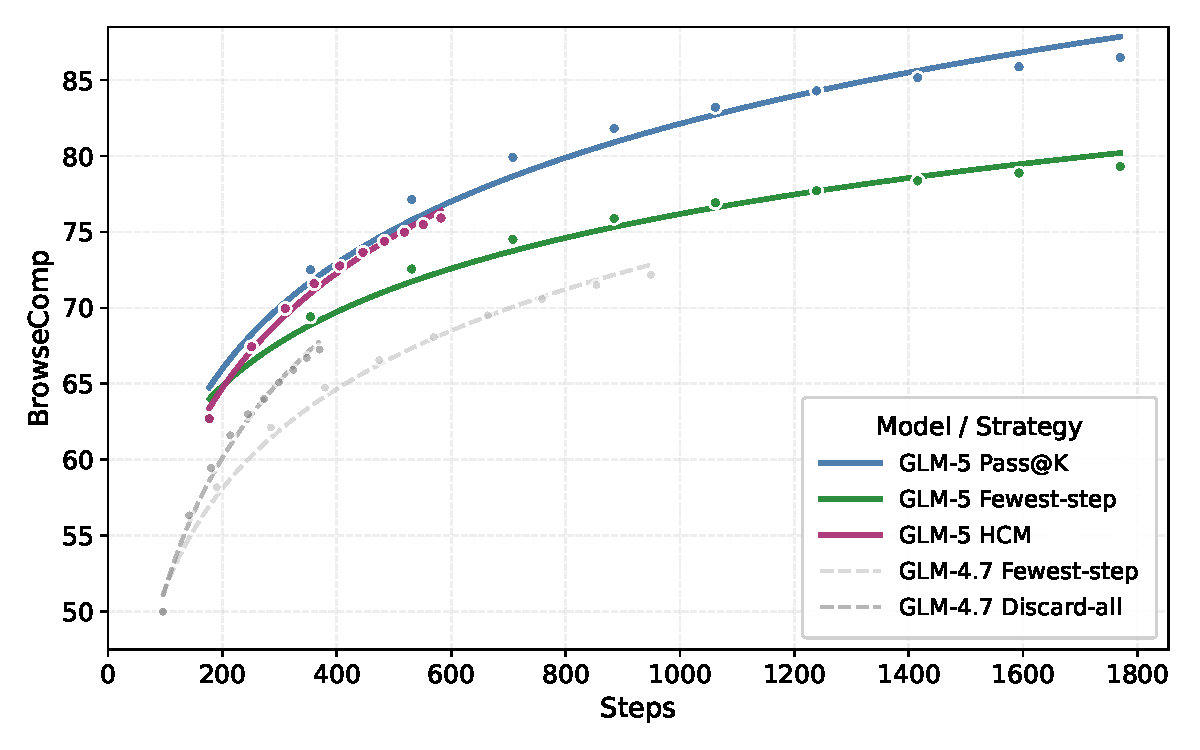
\includegraphics[width=0.7\linewidth]{figures/GLM5-BC-cm.pdf}
    \caption{从 GLM-4.7（灰色基线）到 GLM-5（彩色策略），BrowseComp 在不同上下文管理策略下的准确率。 }
    \label{fig:GLM5-BC-CM}
\end{figure}






% \section{Advancing Agentic Quality: The MobileRL Framework}
% \todo{check later}

% To further enhance GLM-5’s capabilities in complex, multi-step environments, we integrate the principles of MobileRL, a framework specifically designed to overcome the challenges of online reinforcement learning (RL) for autonomous agents. While Slime provides the infrastructure for scalability, MobileRL introduces the algorithmic refinements necessary to handle the heavy-tailed task difficulty and sparse rewards inherent in real-world agentic tasks.

% \subsection{ADAGRPO: Difficulty-Adaptive Policy Optimization}
% The core of MobileRL is Difficulty-ADAptive Group Relative Policy Optimization (ADAGRPO). Built upon the GRPO foundation used in GLM-4.5, ADAGRPO introduces three strategic enhancements to stabilize training and improve sample efficiency:

% Difficulty-Adaptive Positive Replay (AdaPR): Mobile environments often suffer from sparse terminal rewards, where successful trajectories for difficult tasks are rare but highly informative. AdaPR maintains a curated buffer of these high-quality, challenging trajectories and balances them with on-policy samples to amplify the learning signal and stabilize policy updates.

% Failure Curriculum Filtering (FCF): To prevent the model from wasting computational budget on persistently unsolvable "dead-end" tasks, FCF uses online statistics to down-weight extremely difficult instances. This curriculum-based approach reallocates resources toward feasible but challenging tasks, significantly improving overall sample efficiency.
% x
% Shortest-Path Reward Adjustment (SPA): In multi-turn agentic tasks, standard rewards often fail to penalize verbosity. SPA reshapes the reward function by assigning higher returns to shorter, more efficient solutions. This aligns the model’s behavior with user preferences for speed and efficiency, particularly in real-world coding and GUI navigation.


% \subsection{Two-Stage Reasoning Warm-up}
% Before initiating online RL, MobileRL employs a two-stage Supervised Fine-Tuning (SFT) process to ensure a robust policy initialization:

% Reasoning-Free SFT: Builds a strong foundational action space from expert demonstrations.

% Reasoning SFT: Adds intermediate reasoning traces to improve instruction following, multi-step coordination, and policy transparency.

% \subsection{Empirical Results and State-of-the-Art Performance}
% Integrating MobileRL’s ADAGRPO into the GLM series (e.g., MobileRL-9B based on GLM-4V) has yielded significant performance leaps across major benchmarks.

% Table 2: Success Rates on Mobile Agentic Benchmarks  | Model | AndroidWorld | AndroidLab | | :--- | :--- | :--- | | GPT-4o (2024-11) | 34.5% | 31.2% | | UI-Tars-1.5 (355B) | 64.2% | 38.3% | | MobileRL-9B (Ours) | 80.2% | 53.6% |

% The application of ADAGRPO consistently improves performance across all task complexity levels, with the most substantial relative gains observed in high-complexity tasks (Complexity Level 3+). Furthermore, the introduction of SPA has been shown to consistently reduce the number of steps required for task completion, confirming its effectiveness in optimizing for agentic efficiency.

\subsubsection{幻灯片生成}

我们采用自我提升流水线，目标是通过强化学习与拒绝采样微调训练专门的幻灯片生成专家，从而系统性提升幻灯片生成性能。我们先用监督微调（SFT）初始化模型的基础幻灯片生成能力，然后在常见审美与结构属性驱动的多层级奖励下执行强化学习。该阶段显著提升了生成质量。随后我们进行拒绝采样微调与掩码微调，使强化学习获得的知识回注训练语料。该流程以协同迭代方式同时提升数据质量与模型能力。

我们提出 \textbf{多层级奖励构造}，将基于 HTML 的幻灯片生成过程中的奖励信号划分为三层：

\textbf{Level-1：静态标记属性。} 该层关注生成 HTML 中的声明式属性，包括位置、间距、颜色、字体、饱和度等样式属性。基于专业设计原则，我们设计了一组规则来约束模型在生成这些声明时的行为。这些规则既保证生成 HTML 的语法可解析性，也将标记级设计空间约束在更利于表现力、结构清晰度、视觉和谐与可读性的子空间。此外，我们引入了幻觉图片与重复图片检测机制，以抑制幻觉或冗余图像。

\textbf{Level-2：运行时渲染属性。} 与静态检查不同，该层评估渲染过程中 DOM 节点的运行时属性，如元素宽高、边界框及其他几何布局指标。通过约束这些属性，我们鼓励生成幻灯片在空间组织上更符合人类审美偏好。我们开发了分布式渲染服务，能够高吞吐执行渲染任务并提取所需运行时属性。训练中我们观察到多种奖励作弊行为，例如对超长内容硬截断或过度操控间距（见图~\ref{fig:reward_hacking}）。为缓解这些问题，我们改进了渲染器实现，消除可利用漏洞，确保奖励信号真正激励审美一致布局，而非对几何指标的表面迎合。

\begin{figure*}[!thp]
    \centering % 将图居中
    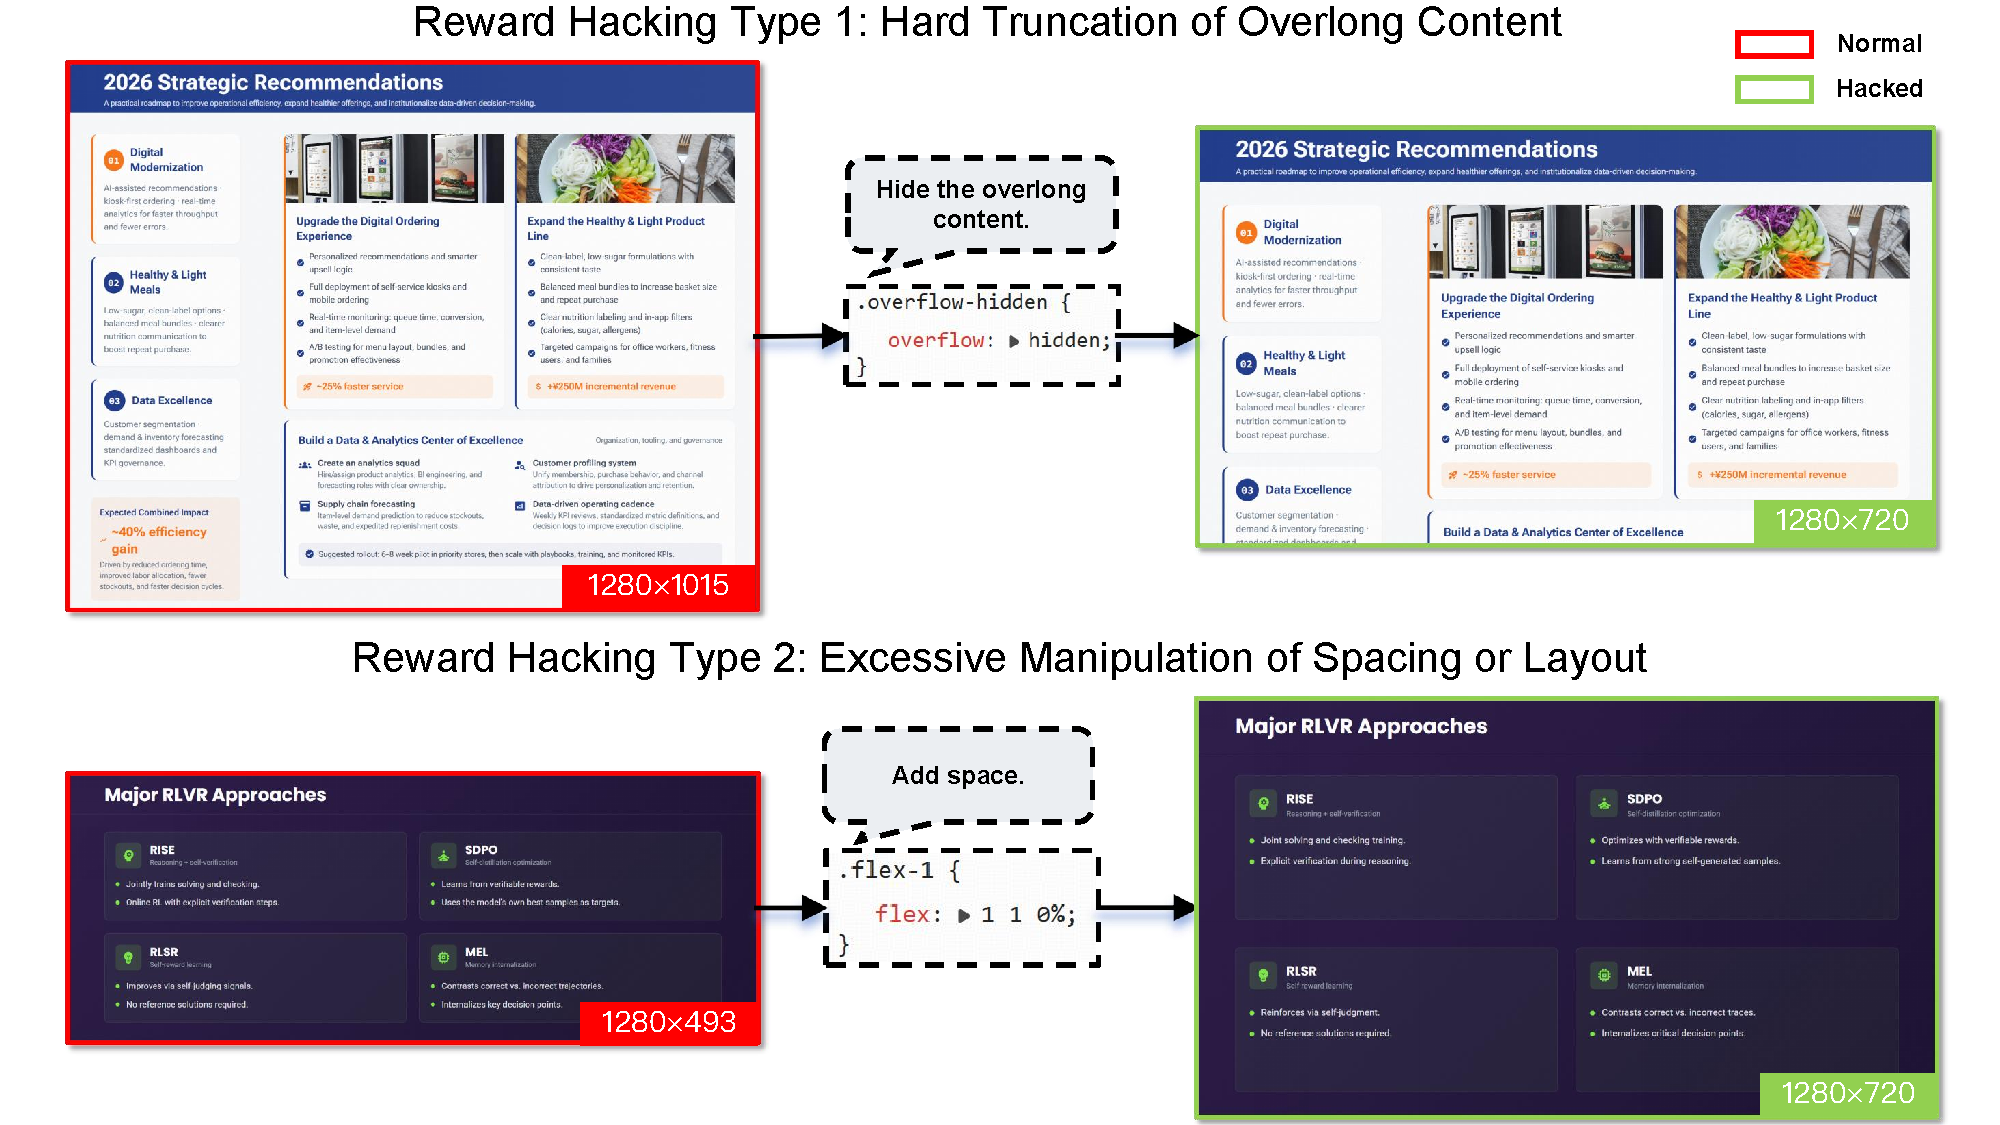
\includegraphics[width=\linewidth]{figures/ppt_reward_hacking.pdf}
   \vspace{-0.1cm}
    \caption{
    幻灯片 RL 训练中的奖励作弊示例。我们的运行时渲染可获取真实属性值，使评估对这类作弊行为更稳健。
    }
    \label{fig:reward_hacking}
    \vspace{-0.2cm}
\end{figure*}

\textbf{Level-3：视觉感知特征。} 在运行时渲染约束之外，我们引入对渲染结果的感知层评估。例如，我们检测异常留白模式作为辅助信号，进一步改善整体构图平衡与视觉美感。

\textbf{训练策略。} 训练中联合优化上述信号，以提升生成 HTML 的结构有效性、增强布局组织并提升整体视觉审美质量。除奖励设计外，我们还通过动态采样重塑训练分布。具体地，以概率方式丢弃部分结构过于简单样本，使优化聚焦更具挑战性的页面并提升复杂构图场景鲁棒性。我们还采用 token 级 policy gradient loss 稳定优化~\cite{yu2025dapo}。此外，我们引入平衡策略，将同一样本不同 rollout 结果分配到多个训练 batch，以降低优化偏差并提升训练稳定性。


\paragraph{拒绝采样。}
在拒绝采样阶段，RL 中使用的奖励函数被迁移到数据过滤流水线，以构建高质量训练子集。
页面级过滤标准包括代码有效性与可编译性；轨迹级进一步约束工具执行正确性与全局内容多样性，以确保结构一致性。
我们采用 Best-of-$N$ 选择策略，即从多个独立生成候选中保留质量最高样本。该机制可有效将分布重加权到更高质量样本，从而提升样本效率与训练稳定性。

\paragraph{基于掩码的细化。} 
尽管拒绝采样可移除大多数低质量输出，但部分轨迹缺陷仅局限于少数页面。若直接丢弃这类样本，会降低有效数据利用率并提高生成成本。为此，我们引入基于掩码的修正机制，自动识别缺陷页面并进行掩码处理，同时保留同一轨迹中的高质量内容。该选择性细化可保留有价值监督信号、提升有效数据效率并减少冗余再生成开销，从而提高整体训练效率。

\paragraph{实证提升。}
严格符合 16:9 宽高比的生成页面占比从 40\% 提升至 92\%，并伴随页面溢出案例显著下降。人工评测进一步显示，相较 GLM-4.5，GLM-5 在内容质量、布局合理性与视觉美感上的胜率分别达到 60\%、57.5\%、65\%，总体胜率达 67.5\%。这些结果为所提出多层级奖励设计与自我提升框架的有效性提供了实证支持。
